\subsection{External Interface Requirements}
This section provides a detailed description of all inputs and outputs from the system. It also gives a description of the hardware, software and communication interfaces and provides basic prototypes of the user interface.

\subsubsection{User Interfaces}
In this section we present the mockups of the GUI.

Figure \ref{fig:login} shows the login page where it's possible to access the registration form for new users.
 \begin{figure}[H]
		\centering
      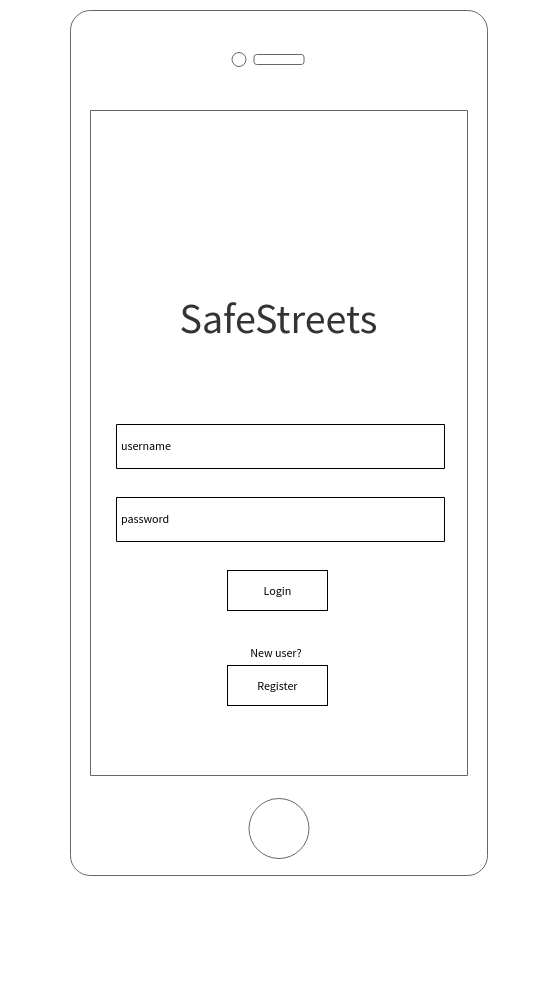
\includegraphics[width=0.5\textwidth]{GUI/login.png}
      \caption{[GUI] Login screen}   \label{fig:login}
\end{figure}

After login the user will enter by default into the first tab "Report", see Figure \ref{fig:takepic}, where is shown what the camera is recording and the user can start taking the picture of the violation.
For the first time a user logs in some banner can appear showing each function of the app. Also we show on the screen some useful reminders about how the picture to be submitted should be.
\begin{figure}[H]
		\centering
      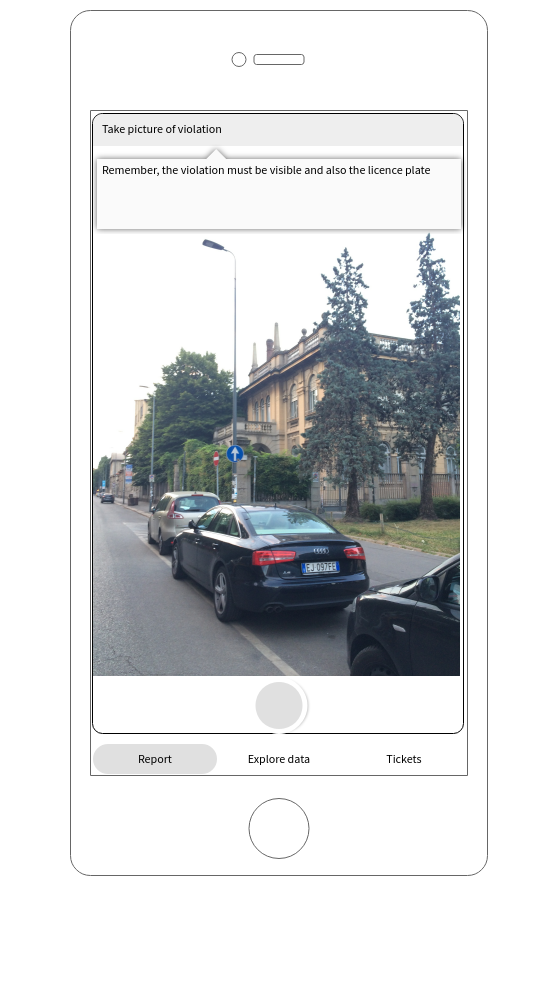
\includegraphics[width=0.5\textwidth]{GUI/takepic.png}
      \caption{[GUI] Report | open camera view}   \label{fig:takepic}
\end{figure}

After the picture has been taken, the apps shows it as in Figure \ref{fig:pictaken} and a "brush tool" will appear, which can be used to cover any other plate appearing in the picture, not related to the veichle being reported.
\begin{figure}[H]
		\centering
      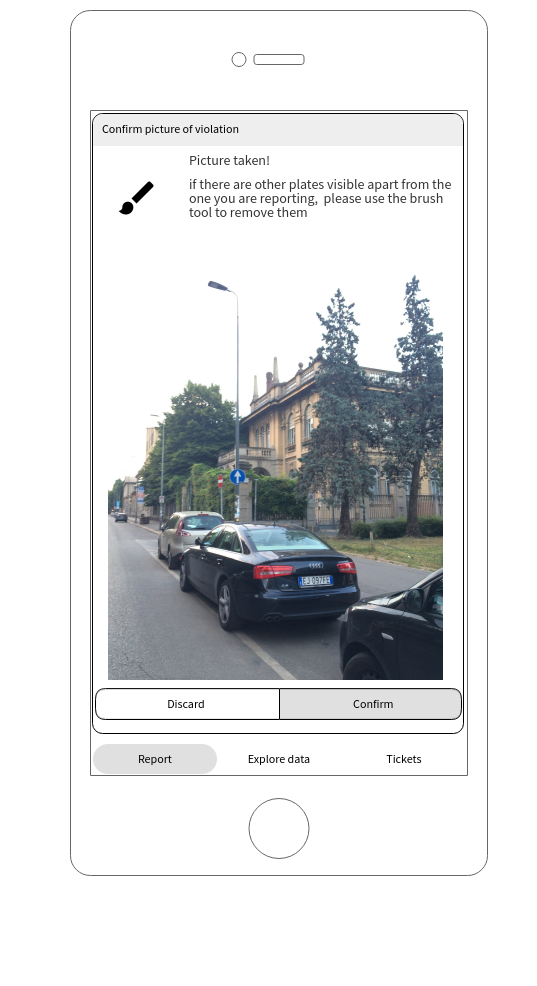
\includegraphics[width=0.5\textwidth]{GUI/picturetaken.png}
      \caption{[GUI] Report | picture of violation taken screen}   \label{fig:pictaken}
\end{figure}

Figure \ref{fig:fillform} shows how appears the form where the user has to select the kind of violation he is rporting from a scroll-down list. Each row has an info button, when pressed the GUI will show a verbal description of the violation related.
\begin{figure}[H]
		\centering
      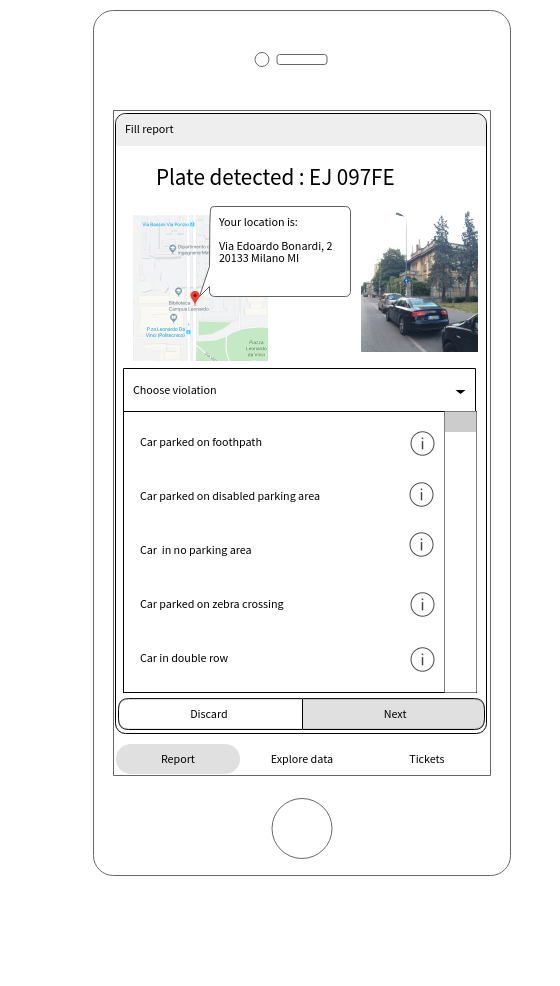
\includegraphics[width=0.5\textwidth]{GUI/fillform.png}
      \caption{[GUI] Report | violation info form screen}   \label{fig:fillform}
\end{figure}

Figure \ref{fig:offenders} shows the view of the plates which have committed the highest number of violations.
\begin{figure}[H]
		\centering
      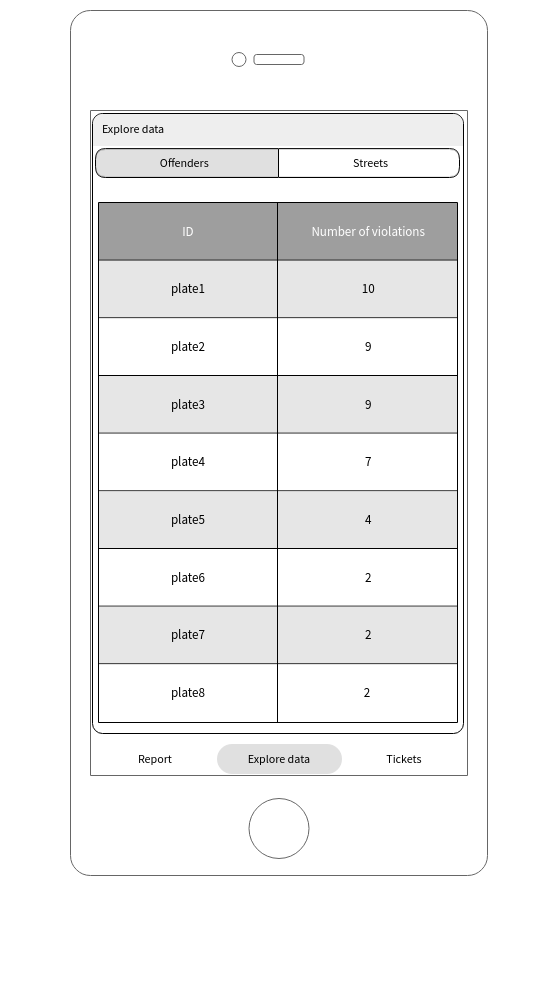
\includegraphics[width=0.5\textwidth]{GUI/offenders.png}
      \caption{[GUI] Explore data screen | offenders}   \label{fig:offenders}
\end{figure}

Figure \ref{fig:heatmap} shows the view of the heatmap, with a map generated by the external API with the colored overlay which represents the number of violation occurred.
\begin{figure}[H]
		\centering
      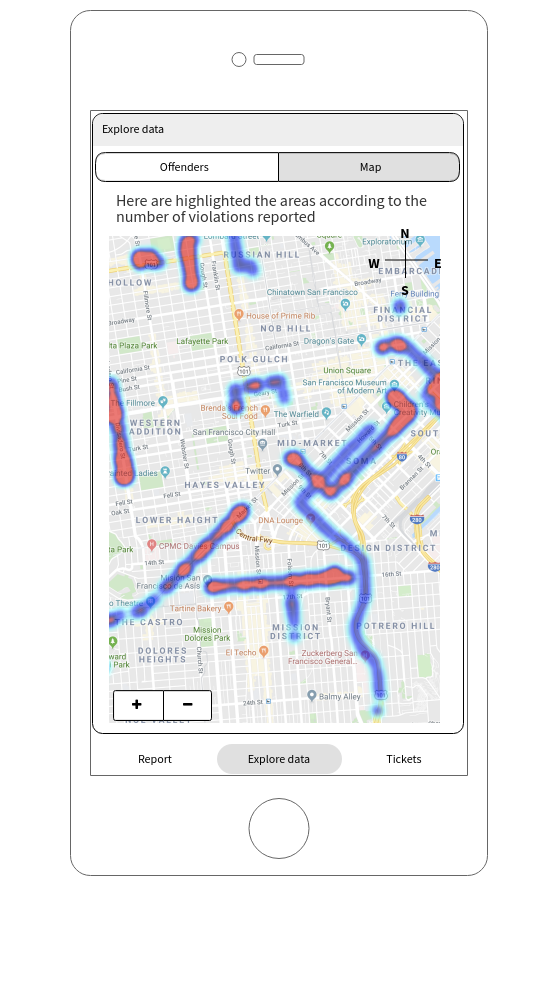
\includegraphics[width=0.5\textwidth]{GUI/heatmap.png}
      \caption{[GUI] Explore data | heatmap}   \label{fig:heatmap}
\end{figure}

Figure \ref{fig:ticket} shows the interface only available to Authority Users where are listed all the tickets that are pending for approval. For each ticket all the key informations are sgown: picture, location, plate, code of the violation.
\begin{figure}[H]
		\centering
      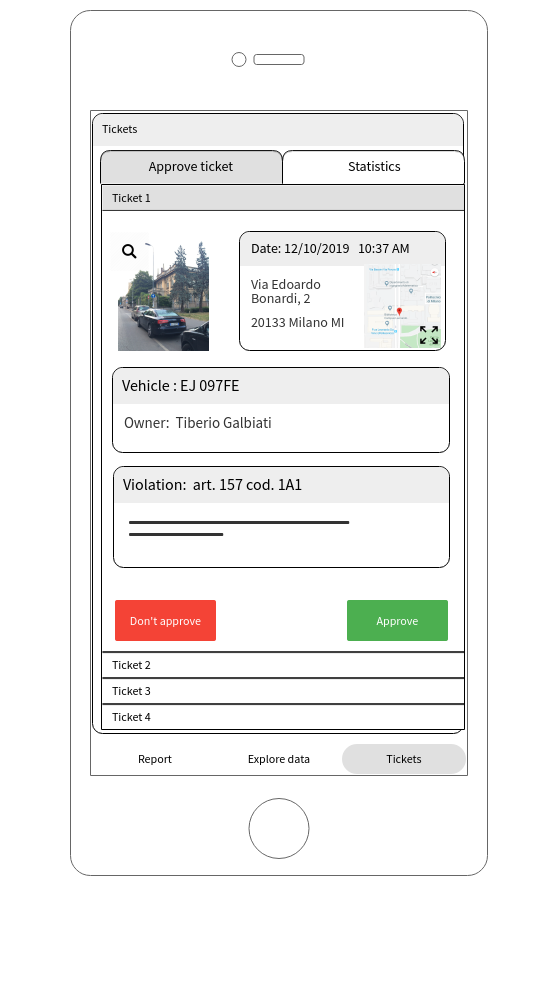
\includegraphics[width=0.5\textwidth]{GUI/ticketapp.png}
      \caption{[GUI] Ticket | approval screen}   \label{fig:ticket}
\end{figure}

\subsubsection{Hardware Interfaces}
there is no need to have hardware interfaces since we are developing a mobile application with a server side.
Iternet connection, GPS, and camera are all managed by the OS of the smartphone where the application will run.
\subsubsection{Software Interfaces}

\subsubsection{Communication Interfaces}


\subsection{Functional  Requirements}
The functional requirements are those which are the fundamental actions of the system. Here we present for every goal a list  of related requirements and domain assumption.
Evrey function shoud work olnly after succesful login.

\begin{itemize}
\item \textbf{[G1] Allow users to notify authorities about traffic violations} %%%%%%%%%%%%%%%%%%%%
\begin{itemize}
  \dom{1} Device has a working internet connection
  \dom{8} The number and kind of violations should be finite (defined by the law)
  \req{1} User must be able to choose the kind of violation from a list
  \req{2} User must be able to read detailed information about each kind of violation he can report
  \end{itemize}

\item \textbf{[G2] Allow users to send pictures with metadata of violations } %%%%%%%%%%%%%%%%%%%%%%%%%%%%%%%
\begin{itemize}
  \dom{2} Device has a camera accessible via software
  \dom{3} The device should acquire position with an accuracy of enouth meters in order to univocally determine the road (e.g. 5 meters)
  \dom{4} We have access to an ALPR service which is able to read every licence plate in a picture and return each of them as a string
  \dom{5} ALPR service has an accuracy of more than 95\%
  \dom{6} The device should take pictures with enough resolution to be able to read by the ALPR service
  \dom{7} Every vehicle that can be reported should have a licence plate visible
  \req{3} Date, time and position should be automatically added to the violation reported
  \req{4} We should require the user to send again a picture in case the plate is not visible
  \req{5} The user must be able to select the veichle to report in case there are other veichles in picture
  \req{6} Application must automatically determine the street name where User is
\end{itemize}

\item \textbf{[G3] Allow users to mine information recorded}  %%%%%%%%%%%%%%%%%%%%%%%%%%%%%%%%%%%
\begin{itemize}
  \req {7} Application must be able to count occurrency of violations
  \req {8} Application must be able to count violation for each veichle
  \req {9} Application should show the all the veichles ordered with the number of violations
  \req {10} Application should visualize the areas where violation occurred
  \req {11} Application must use a gradient of color to show the occurrencies of violations as an overlay of a interactive map
\end{itemize}

\item \textbf{[G4] Have at least two different priviledge for mining data} %%%%%%%%%%%%%%%%%%%%%
\begin{itemize}
  \dom{9} Every authority account is verified and it's not possible to be created using the front end
  \req {12} Regular endusers can see the list of veichles with the highest number of violations but they cannot see the actual licence plate, instead of that a generic identifier is shown
  \req{13} Authority users can know the exact licence plate when mining data about offenders
  \req{14} Only authority users can access the ticket approval section
\end{itemize}

\item \textbf{[G5] Generate traffic tickets}
\begin{itemize}
  \dom{10} We have access to the vehicle registration database where are stored licence plates, names and the addresses of the owners of every vehicle registered
  \dom{11} We have access to a database where are stored all the codes of violations and the amount of fine for the violation
  \req {15} Application must be able to read every violation stored and automatically generate a ticket
  \req {16} application showld offer to authorities the possibility to approve tickets or not
\end{itemize}

\item \textbf{[G6] Generate statistics about issued tickets}
\begin{itemize}
  \req{17} Application must store all the tickets created
  \req{18} Application must read all the history of tickets created
\end{itemize}

\item \textbf{[G7] Be sure every information uploaded is never altered}
\begin{itemize}
 \dom{12} The only way to upload pictures of violation is thuough the application
 \req{19} The application must be able to know if a picture has been altered
 \req{20} If a picture has been altered the applcation must automatically flag as not valid the corresponding ticket
\end{itemize}

\end{itemize}}


\subsubsection{Use Cases diagrams}
Here are presented the use case diagrams for each main function. In the next section each use case will be verbally presented.

%%%%big pict here %%%%%%%%%%%%
%%%%%%Basic Service UseCase diagram
 \begin{figure}[H]
		\centering
      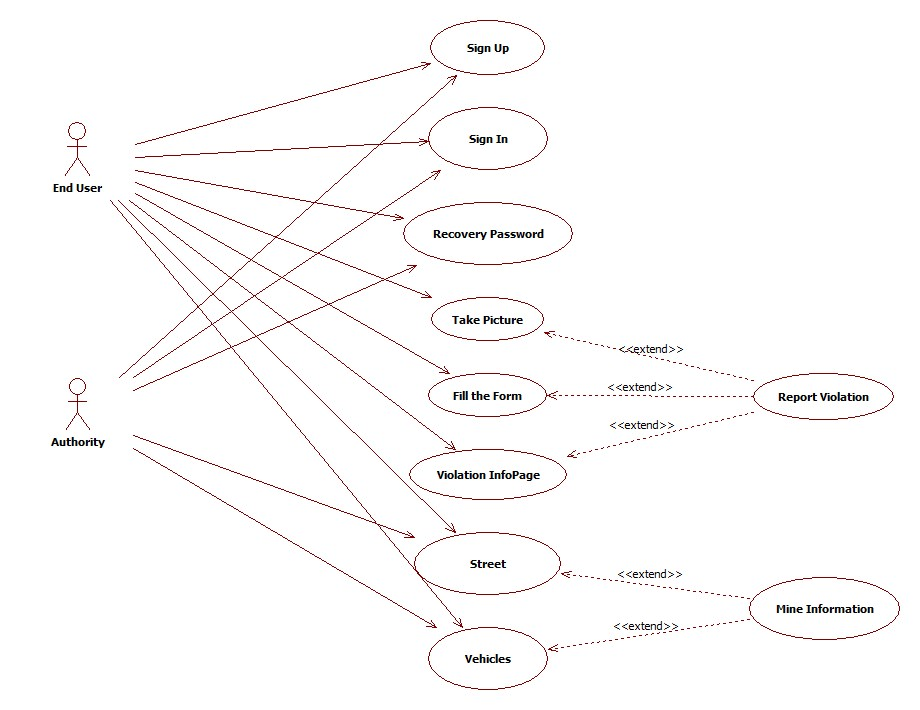
\includegraphics[width=0.8\textwidth]{Images/BasicServiceUseCase.jpg}
      \caption{Basic service use case diagram}   \label{fig:BasicService}
\end{figure}

  %%%%%%Advanced Function UseCase diagram
 \begin{figure}[H]
		\centering
      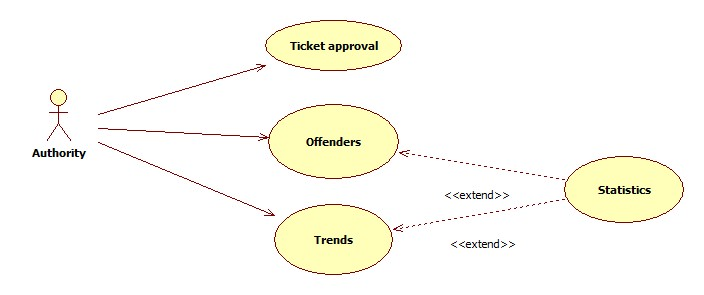
\includegraphics[width=0.8\textwidth]{Images/AdvancedFUnUseCase.jpg}
      \caption{Advanced function use case diagram}   \label{fig:AdvancedFunction}
\end{figure}


\subsubsection{Use Cases Description}
In the following section a description of each use case is provided. For every use case is reported: an ID defining each case, the entry conditions, the steps to accomplish the exit condition and any exception that may occur. \\


%%%%%%%USE CASES HERE ***********************************************************************
%%%%Basic service use case definition
	\textbf{ID}: \ucas{1} \\
	\textbf{Name}: Sign-Up \\
	\textbf{Actor}: Guest \\
	\textbf{Entry conditions}:
	\begin{enumerate}
		\item{A citizen who wants to use the service}
	\end{enumerate}
	\textbf{Event flow}:
	\begin{enumerate}
		\item{The guest reaches the registration page containing the relative form}
		\item{The guest fills up the form and clicks on "Sign up" to complete the process}
		\item{The system redirects the user to his profile page and sends a confirmation email}
	\end{enumerate}
	\textbf{Exit conditions}:
	\begin{itemize}
		\item{The guest has successfully registered in the system}
	\end{itemize}
	\textbf{Exceptions}:
	\begin{enumerate}
    		\item{The guest left an empty field or typed something wrong. So an error message is displayed and the user is asked to fill the form again}
 	   \end{enumerate}
	\rule{\linewidth}{0.4pt}
  %%%%%%%%%%%%%%%%%%%%%%%%%%%%%%%%%%%%%%%%%%%%%%%%%%%%%%%%%%%%%%%%%%%%%%%
	\textbf{ID}: \ucas{2} \\
	\textbf{Name}: Login \\
	\textbf{Actor}: User \\
	\textbf{Entry conditions}:
	\begin{enumerate}
		\item{The user has already registered}
	\end{enumerate}
	\textbf{Event flow}:
	\begin{enumerate}
		\item{The user reaches the login page containing the relative form}
		\item{The user types the username and password in the login form and clicks on ”Login” button}
		\item{The system redirects the user to the application homepage}
	\end{enumerate}
	\textbf{Exit conditions}:
	\begin{itemize}
		\item{The user has access to the application functionalities}
	\end{itemize}
	\textbf{Exceptions}:
	\begin{enumerate}
    		\item{Username and password didn’t correspond or the username didn’t exist so an error message is displayed and the user is asked to fill the login form again}
 	   \end{enumerate}
	\rule{\linewidth}{0.4pt}
  %%%%%%%%%%%%%%%%%%%%%%%%%%%%%%%%%%%%%%%%%%%%%%%%%%%%%%%%%%%%%%%%%%%%%%%
	\textbf{ID}: \ucas{3}  \\
	\textbf{Name}: Recover Password \\
	\textbf{Actor}: User \\
	\textbf{Entry conditions}:
	\begin{enumerate}
		\item{The user has already registered}
	\end{enumerate}
	\textbf{Event flow}:
	\begin{enumerate}
		\item{The user reaches the login page containing the relative form}
		\item{The user clicks on ”Password recovery” button and is redirected to the password recovery page.}
		\item{The user inserts his email and clicks on ”Reset password”}
		\item{The system sends an email to the user with a link and instruction to reset the password}
		\item{The user chooses and types a new password and confirms}
		\item{The application check whether the entered password is strong enough or not}
		\item{The system redirects the user to the login page}
	\end{enumerate}
	\textbf{Exit conditions}:
	\begin{itemize}
		\item{The user has changed his password}
	\end{itemize}
	\textbf{Exceptions}:
	\begin{enumerate}
    		\item{The inserted email doesn't match any user in the database so it is displayed an error message and the user is asked to retype a valid email}
 	   \end{enumerate}
	\rule{\linewidth}{0.4pt}
  %%%%%%%%%%%%%%%%%%%%%%%%%%%%%%%%%%%%%%%%%%%%%%%%%%%%%%%%%%%%%%%%%%%%%%%
  \textbf{ID}: \ucas{4a} \\
  \textbf{Name}: Report a violation - taking picture \\
  \textbf{Actor}: User   \\
  \textbf{Entry conditions}:
  \begin{enumerate}
    \item{User is logged in}
  \end{enumerate}
  \textbf{Event flow}:
  \begin{enumerate}
    \item{User enters the section "Report a violation"}
    \item{System opens the camera of smartphone and ask user to take a picture of the violation}
    \item{The system reminds the user: the violation and the licence plate of the vehicle which is in violation must be visible }
    \item{The user takes the picture }
    \item{The system shows the picture just taken }
    \item{The system asks the user: if there are other plates visible in the picture, which are not the one of the vehicle to be reported, use the finger to delete them }
    \item{The system shows "brush tool mode" and the user can cover the other licence plates whith his finger. User can skip this part if there are no other plates}
    \item{When done, user press continue button }
    \item{The system sends the picture to the ALPR service which returns the string containing the plate decoded. User just waits}
    \item{The system shows now on the screen the "Report violation form"}
  \end{enumerate}
  \textbf{Exit conditions}:
  \begin{enumerate}
    \item{User must continue to next \ucas{4b}}
  \end{enumerate}
  \textbf{Exceptions}:
  \begin{enumerate}
    \item{If no plate is found, the user has to repeat this use case, starting from taking the picture again}
    \item{If the ALPR service returns more than one plate, the user is informed that must delete the not required plates and the system goes again to the "brush tool mode"}
    \item{If user doesn't continue to the next use case: e.g. presses exit button, or closes the app for more than 10 minutes, the picture taken is discarded}
  \end{enumerate}
  \rule{\linewidth}{0.4pt}
  %%%%%%%%%%%%%%%%%%%%%%%%%%%%%%%%%%%%%%%%%%%%%%%%%%%%%%%%%%%%%%%%%%%%%%%
  \textbf{ID}: \ucas{4b} \\
  \textbf{Name}: Report a violation - fill the form \\
  \textbf{Actor}: User   \\
  \textbf{Entry conditions}:
  \begin{enumerate}
    \item{User has successfully completed the precedent \ucas{4a}}
    \item{User is in the fill-form section of the app}
  \end{enumerate}
  \textbf{Event flow}:
  \begin{enumerate}
    \item{The system sends GPS location to the external service to get the complete address of the user}
    \item{The form is pre-filled with the address that is given by the external service}
    \item{The user must choose from a list of violations the one referred to the picture taken which wants to report. In the UI every row contains the name of the violation and a "info" button}
    \item{The user choose to send the form}
  \end{enumerate}
  \textbf{Exit conditions}:
  \begin{enumerate}
    \item{The violation is correctly inserted and stored}
  \end{enumerate}
  \textbf{Exceptions}:
  \begin{enumerate}
		\item{If user doesn't send the form: e.g. presses exit button, or closes the app for more than 10 minutes, the violation reported is discarded}
  \end{enumerate}
  \rule{\linewidth}{0.4pt}
  %%%%%%%%%%%%%%%%%%%%%%%%%%%%%%%%%%%%%%%%%%%%%%%%%%%%%%%%%%%%%%%%%%%%%%%
  \textbf{ID}: \ucas{4b1} \\
  \textbf{Name}: Report a violation - fill the form - violation infopage \\
  \textbf{Actor}: User   \\
  \textbf{Entry conditions}:
  \begin{enumerate}
    \item{User is in Use case \ucas{4b} }
    \item{User has pressed the "info" button of a violation from the list }
  \end{enumerate}
  \textbf{Event flow}:
  \begin{enumerate}
    \item{System shows a brief decriprion of the selected violation}
  \end{enumerate}
  \textbf{Exit conditions}:
  \begin{enumerate}
    \item{User goes back to Use case \ucas{4b}}
  \end{enumerate}
  \textbf{Exceptions}:

  \rule{\linewidth}{0.4pt}
  %%%%%%%%%%%%%%%%%%%%%%%%%%%%%%%%%%%%%%%%%%%%%%%%%%%%%%%%%%%%%%%%%%%%%%
	\textbf{ID}: \ucas{5a} \\
	\textbf{Name}: Mine information - street heatmap \\
	\textbf{Actor}: User  \\
	\textbf{Entry conditions}:
	\begin{enumerate}
		\item{User is logged in}
	\end{enumerate}
	\textbf{Event flow}:
	\begin{enumerate}
		\item{User enters the section "Explore data"}
    \item{The user chooses to get the map about streets with the highest frequency of violations}
    \item{The system retrieves data from the database of violations, counting for each street the number of occurrencies}
    \item{The system sends to the external maps API the count of violation and the road name/coordinates}
    \item{The app shows the map with an overlay which higlights the areas with a gradient color according to the number of violations occurred}
	\end{enumerate}
	\textbf{Exit conditions}:
	\begin{\begin{enumerate}
		  \item{User wants to go back to "Explore data" area}
	\end{enumerate}
	\textbf{Exceptions}:
  \begin{enumerate}
    \item{If there are no records the app will report no data available message}
  \end{enumerate}
	\rule{\linewidth}{0.4pt}
  %%%%%%%%%%%%%%%%%%%%%%%%%%%%%%%%%%%%%%%%%%%%%%%%%%%%%%%%%%%%%%%%%%%%%%%
	\textbf{ID}: \ucas{5b} \\
	\textbf{Name}: Mine information - offenders \\
	\textbf{Actor}: AuthorityUser   \\
	\textbf{Entry conditions}:
	\begin{enumerate}
		\item{AuthorityUser is logged in}
	\end{enumerate}
	\textbf{Event flow}:
	\begin{enumerate}
		\item{AuthorityUser enters the section "Explore data"}
		\item{The system asks which kind of data the AuthorityUser wants to know}
    \item{The AuthorityUser chooses to get the data about vehicles that committed the highest number of violations}
    \item{The system queries the table where for each licence plate is associated the count of violations }
    \item{The system will report in a tabular way the plate of the vehicle and the count of violations committed}
    \item{If the AuthorityUser scrolls down, the system will offer the chance to load more rows}
	\end{enumerate}
	\textbf{Exit conditions}:
  \begin{enumerate}
    \item{AuthorityUser wants to go back to "Explore data" area}
  \end{enumerate}
	\textbf{Exceptions}:
	\begin{enumerate}
		\item{If there are no records the app will report no data available message}
	\end{enumerate}
	\rule{\linewidth}{0.4pt}
  %%%%%%%%%%%%%%%%%%%%%%%%%%%%%%%%%%%%%%%%%%%%%%%%%%%%%%%%%%%%%%%%%%%%%%%
\item \textbf{Advanced function}\\
		\textbf{ID}: \ucas{6} \\
		\textbf{Name}: Ticket approval  \\
		\textbf{Actor}: AuthorityUser   \\
		\textbf{Entry conditions}:
		\begin{enumerate}
			\item{A new violation is inserted in database}
      \item{AuthorityUser logged in}
		\end{enumerate}
		\textbf{Event flow}:
		\begin{enumerate}
      \item{Every time a new violation is created by a EndUser the system will create automatically a ticket to be approved}
			\item{AuthorityUser enters the section "Tickets"}
			\item{AuthorityUser enters the section "Approve Tickets"}
      \item{The System will show the list of tickets available for approval }
      \item{AuthorityUser selects one ticket and system will show the related details}
      \item{System will ask the AuthorityUser if he wants to approve or not the ticket}
  		\end{enumerate}
		\textbf{Exit conditions}:
    \begin{enumerate}
      \item{User wants to go back to "Ticket" area}
      \item{AuthorityUser approves the ticket}
      \item{AuthorityUser doesn't approve the ticket}
    \end{enumerate}
		\textbf{Exceptions}:
		\begin{enumerate}
			\item{If there aren't tickets pending, the app will report a message saying that there aren't new tickets to approve}
		\end{enumerate}
		\rule{\linewidth}{0.4pt}
    %%%%%%%%%%%%%%%%%%%%%%%%%%%%%%%%%%%%%%%%%%%%%%%%%%%%%%%%%%%%%%%%%%%%%%%%%%%
    \textbf{ID}: \ucas{7} \\
    \textbf{Name}: Statistics - tickets offenders \\
    \textbf{Actor}: AuthorityUser   \\
    \textbf{Entry conditions}:
    \begin{enumerate}
      \item{AuthorityUser logged in}
    \end{enumerate}
    \textbf{Event flow}:
    \begin{enumerate}
			\item {AuthorityUser enters the section "ticket statistics"}
			\item {The system will show the available ticket statisics options available to show}
			\item {AuthorityUser selects to see the statistics about offenders }
      \item {The system queries the table about all tickets, getting the count of tickets associated to every citizen present in the database of ticket created}
      \item {The system will report in a tabular way the name of the citizen and the count of approved tickets he has received}
      \item {If the AuthorityUser scrolls down, the system will offer the chance to load more rows}
    \end{enumerate}
    \textbf{Exit conditions}:
    \begin{enumerate}
      \item{The AuthorityUser wants to go back to other sections}
    \end{enumerate}
    \textbf{Exceptions}:
    \begin{enumerate}
    \end{enumerate}
    \rule{\linewidth}{0.4pt}
    %%%%%%%%%%%%%%%%%%%%%%%%%%%%%%%%%%%%%%%%%%%%%%%%%%%%%%%%%%%%%%%%%%%%%%%
    \textbf{ID}: \ucas{5} \\
    \textbf{Name}: Statistics - trends \\
    \textbf{Actor}: AuthorityUser   \\
		\textbf{Entry conditions}:
    \begin{enumerate}
      \item{AuthorityUser logged in}
    \end{enumerate}
    \textbf{Event flow}:
    \begin{enumerate}
			\item {AuthorityUser enters the section "ticket statistics"}
			\item {The system will show the available ticket statisics options available to show}
      \item {AuthorityUser has chosen to see the Statistics - trend option}
			\item {The system shows the count of the approved tickets of last month}
			\item {The system shows the ratio of tickets approved over the total number of violations reported}
    \end{enumerate}
    \textbf{Exit conditions}:
    \begin{enumerate}
			\item The AuthorityUser wants to go back to other sections
    \end{enumerate}
    \textbf{Exceptions}:
    \begin{enumerate}
    \end{enumerate}
    \rule{\linewidth}{0.4pt}


\subsubsection{Requirements traceability matrix}

\begin{table}[] 
\begin{tabular}{|l|l|}
\hline
\textbf{Requirement} & \textbf{Use Case} \\ \hline
[R1]                   &    \ucas{4b}    \\ \hline  %%choose kind
[R2]                   &    \ucas{4b1}    \\ \hline %%read info
[R3]                   &    \ucas{4b}    \\ \hline  %%date time loc autoadded
[R4]                   &    \ucas{4a}    \\ \hline %%plate not visible
[R5]                   &    \ucas{4a}    \\ \hline %%brushtool
[R6]                   &    \ucas{4b}    \\ \hline  %%streetname
[R7]                   &    \ucas{5a}    \\ \hline %% count violations strt
[R8]                   &    \ucas{5b}  \ucas{5c}  \\ \hline %% count violations off
[R9]                   &    \ucas{5b}  \ucas{5c}   \\ \hline
[R10]                   &    \ucas{5a}    \\ \hline %%hetatmap
[R11]                   &    \ucas{5a}    \\ \hline %%heatmap gradient
[R12]                   &    \ucas{}    \\ \hline %%endus genericiUUID
[R13]                   &    \ucas{}    \\ \hline %%authority see plate
[R14]                   &    \ucas{}    \\ \hline %%ticket approval
[R15]                   &    \ucas{}    \\ \hline %%genticket
[R16]                   &    \ucas{}    \\ \hline %%ticket approval
[R17]                   &    \ucas{}    \\ \hline %%tick Stats
[R18]                   &    \ucas{5a}    \\ \hline %%tick stst again
[R19]                   &    \ucas{5a}    \\ \hline %%picaltered
[R20]                   &    \ucas{5a}    \\ \hline %%picaltered flagging
\end{tabular}
\end{table}



\subsection{Performance Requirements}

\subsection{Design Constraints}%%%%%%%%%%%%%%%%%%%T.

\subsubsection{Standards compliance}
The app shoudld be available for the two main operating systems of smartphones: Android Os and Apple iOS.\\



\subsubsection{Hardware limitations}
The app will have a server side and a client side (smartphone).
On server side limitations can be the size of available storage and the bandwidth.
On smartphone side we have the network connectivity (3G/4G connection) and GPS limitations in some areas.

\subsubsection{Any other constraint}
Application should be compliant to European GDPR.\\
The traffic violations which can be reported should be compliant to the local traffic code where the app will be used.\\
For an use in Italy the app should be compliant to the "Codice della Strada", in particular parking violations are reported in Art. 157.\\

\subsection{Software System Attributes}
\subsubsection{Simple User Interface}
The user interface has to be as simple and intuitive as possible, the application should allow an average user to set up an account and start using the application understanding its functionality in no more than a dozen minutes. In addition there should be a complete tutorial to makes it easy using the application.

\subsubsection{Reliability}
The application provides a reliable service in which individual users can easily log in and report the violations in the most optimal way. Furthermore it Warranties that the chain of custody of the information coming from the users is never broken, and the information is never altered. This would provide a secure and reliable system. In addition, if the license plate	is not readable from the picture the application should warn the user to send an other photo.
\subsubsection{Availability}
The application must offer the maximum availability, granting its service every day at any time (24/7). The lack of service must be minimal.Reporting violation and taking the information about the vioalation coming from SafeStreets must be active every day at any time. The lack of service is acceptable only if it is due to maintenance. In this case, users must receive a warning 48 hours before.
\subsubsection{Security}
The application need to be safe and it does not have particular security concerns except the ones related to unauthorized login. The login of Users and especially of authorities must be very safe to avoid reporting. Moreover, the means of communication must be encrypted to save the confidentiality of information sent to SafeStreets.
\subsubsection{Maintainability}
The application will be maintained and designed in such a way it makes it easier to maintain and it should be understandable for both the users and the authorities. Furthermore, the system will put effort in keeping the live data services (such as highlighting the streets with the highest frequency of violations or the vehicles that commit the most violation) always online.
\subsubsection{Portability}
Portability of user data from a device to another is possible by entering personal login data. Also the application will be able to run for devices with different operating systems.
